\subsubsubsection{Brisanje naloga zaposlenog}

\begin{itemize}
    \item Kratak opis:
        \begin{itemize}
            \item Administrator briše nalog zaposlenog nakon prekida radnog odnosa.
        \end{itemize}
    \item Učesnici:
        \begin{itemize}
            \item Administrator
        \end{itemize}
    \item Preduslovi:
        \begin{itemize}
            \item Administrator poseduje informacije o nalogu korisnika kome briše nalog.
        \end{itemize}
    \item Postuslovi:
        \begin{itemize}
            \item Korisniku je obrisan nalog i baza je ažurirana.
        \end{itemize}
    \item Osnovni tok:
        \begin{enumerate}
         \item Administrator otvara stranicu za pretraživanje sistema.
         \item Administrator unosi korisničko ime naloga koji želi da obriše.
         \item Administrator bira opciju ``Obriši nalog''.
         \item Sistem briše nalog i sve dodatne informacije vezane za obrisani nalog.
         \item Sistem obaveštava administratora o uspešnom brisanju naloga.
        \end{enumerate}
    \item Alternativni tok:
        \begin{itemize}
            \item[4.a] U slučaju greške pri brisanju naloga, sistem obaveštava administratora o neuspelom brisanju i prikazuje mu poruku da pokuša ponovo. Proces se nastavlja od koraka 3.
        \end{itemize}
\end{itemize}

\begin{figure}[H]
\begin{center}
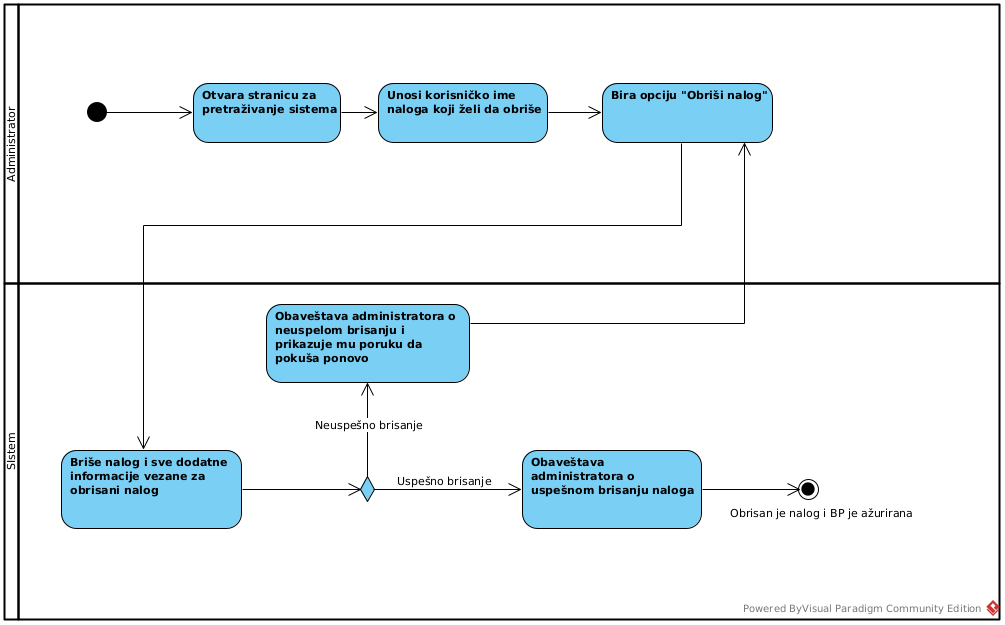
\includegraphics[width=\textwidth]{Pictures/activity_employee_delete.png}
\end{center}
    \caption{Dijagram aktivnosti brisanje naloga usled neadekvatnog korišćcenja od strane klijenta ili prekida radnog odnosa zaposlenog}
\label{fig:ActivityDeleteEmployeeAccount}
\end{figure}
